\chapter{图表示的转换与因子图}
\label{chap:pgm-representations}

同一个联合分布能否既画成有向图，又画成无向图？如果可以，换图以后，从图上读出的条件独立关系是否仍然相同？第~\ref{chap:pgm-directed}章和第~\ref{chap:pgm-undirected}章分别建立了两类图的分解与分离规则，但这两个问题不能只靠删去箭头来回答。例如，用$F,H,A,S$分别表示故障、过热、报警与传感器失灵，则报警模型$F\to H\to A\leftarrow S$中的$F$与$S$是独立根节点；观察报警$A$以后，两条原因路径却可能产生关联。无向图中的条件化只会阻断路径，无法用同一种规则直接复现这种变化。

比较表示时，需要分清三个对象：图结构经过什么转换，转换后的图声明哪些独立性，以及因子乘积怎样被重新组织。保持因子乘积不变，可以保持全部概率查询的答案，却未必使新图继续声明原来的全部独立性。因子图则把关注点进一步移到计算上：它显式记录每个因子需要哪些变量，并不与有向图模型、Markov网络构成互斥的模型分类。本章先建立道德化与弦化这两类结构转换，再比较独立性和因子分解，最后说明因子图怎样保留局部计算结构。

以下图均为有限图，默认在同一节点集合$V$上比较，不引入辅助变量或潜变量。节点$i$对应标量随机变量$X_i$，节点集合$A$对应随机向量$\bm{X}_A$。涉及条件概率表与数值计算时，变量取有限个离散值；连续情形的相应限制会在需要处说明。

\section{有向图与无向图的结构转换}
\label{sec:pgm-representations-structural-conversions}

有向图转成无向图时，不能只擦掉箭头；无向图转成适合定向或消元的结构时，也不能任意添加边。前一种转换要保留共同子节点引起的父节点联系，后一种转换要让删点时留下的邻居已经成团。本节先定义这些操作本身，下一节再判断它们保留了哪些独立性。

\subsection{骨架、祖先图与道德图}
\label{sec:pgm-representations-ancestral-graphs}

d-分离要检查路径中的碰撞点是否被自身或后代的观测激活。若只想回答一个给定查询，可以把这些判断转成一次无向分离，但所用的无向图必须随查询改变。

\begin{definition}[骨架]
  \label{def:pgm-representations-skeleton}
  设$\mathcal{G}=(V,E)$为有限有向图。将每条有向边$i\to j$替换为无向边$\{i,j\}$，所得无向图称为$\mathcal{G}$的\term{骨架}（skeleton），记为$\operatorname{skel}(\mathcal{G})$。骨架保留节点与邻接关系，但丢弃全部箭头方向。
\end{definition}

\begin{definition}[祖先闭包]
  \label{def:pgm-representations-ancestral-closure}
  设$\mathcal{G}=(V,E)$为有限有向图。对$T\subseteq V$，定义
  \[
    \operatorname{an}^{+}(T)=T\cup\bigcup_{i\in T}\operatorname{an}(i),
  \]
  称为$T$的\term{祖先闭包}（ancestral closure）。若$\operatorname{an}^{+}(T)=T$，则称$T$为祖先集。
\end{definition}

祖先闭包收集查询节点及所有能沿有向路径到达它们的节点，上标$+$强调集合包含查询节点自身。它只由有向图和节点集决定，尚未改变边的方向。

\begin{definition}[查询的祖先图]
  \label{def:pgm-representations-query-ancestral-graph}
  设$\mathcal{G}=(V,E)$为有限有向无环图。对两两不交且$A,B$非空的$A,B,S\subseteq V$，令$U=\operatorname{an}^{+}(A\cup B\cup S)$。由$U$中的节点以及原图中两端都位于$U$的边组成的诱导子图$\mathcal{G}[U]$，称为查询$(A,B\mid S)$的\term{祖先图}（ancestral graph）。
\end{definition}

查询的祖先图随$A,B,S$改变。它保留可能参与当前d-分离判断的祖先结构，而不是固定取整个有向图。

\begin{definition}[有向图的道德图]
  \label{def:pgm-representations-moral-graph}
  给定有限有向图$\mathcal{H}$，先在每个节点的任意两个不同父节点之间补一条无向边，再把$\mathcal{H}$中的全部有向边替换为无向边。由补边和原有向边的无向版本共同组成的无向图称为$\mathcal{H}$的\term{道德图}（moral graph），记为$\operatorname{mor}(\mathcal{H})$。这一构造称为\term{道德化}（moralization）。
\end{definition}

道德化把每个节点及其父节点连成团，使同一个局部条件因子的全部变量在无向图中两两相邻。祖先图负责选取与查询相关的节点，道德图负责把所保留的有向局部结构转成无向连接；两步的作用不能互换。

\begin{figure}[htbp]
  \centering
  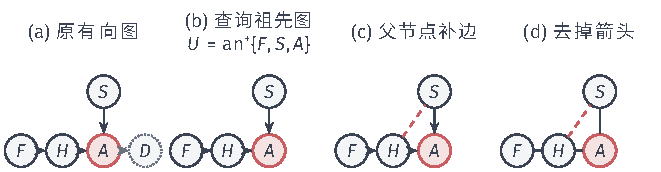
\includegraphics[width=\linewidth]{figures/03-models/03-probabilistic-graphical-models/tikz/pgm-representations-ancestral-moralization/figure.pdf}
  \caption{查询祖先图的道德化过程。原有向图在报警节点$A$后接一个后代$D$；对查询$F\perp S\mid A$，祖先闭包$U=\{F,H,A,S\}$依赖端点和条件集，因而先删去不在$U$中的$D$及其关联边$A\to D$。点线轮廓、点线有向边与$\times$共同标识这些待删元素；随后在共同子节点$A$的父节点$H,S$之间加入的虚线专门编码补边，并用“补$H-S$”直接标注。最后去掉原边的箭头得到查询祖先图的道德图；检测该查询时还要删除条件节点$A$。红色填充并配合“给定”文字标识条件节点。}
  \label{fig:pgm-representations-ancestral-moralization}
\end{figure}

图~\ref{fig:pgm-representations-ancestral-moralization}把四个操作分开显示。点线与$\times$表示祖先闭包会删去的原节点和原边，带“补”标签的虚线表示道德化新增边，两种编码不共享线型语义。读图时应先观察节点集合怎样随查询收缩，再观察$H-S$补边怎样在去掉箭头后保留共同子节点的影响；若换成不包含$A$及其后代的查询，祖先图和后续补边都可能改变。

\subsection{弦化与完美消除序}
\label{sec:pgm-representations-chordal-conversion}

无向图的下一类转换服务于删点与定向。若删去一个节点以后，它尚未删除的邻居并未两两相连，后续计算通常会产生同时依赖这些邻居的新函数；图上需要用新增边记录这种联系。

\begin{definition}[弦图与弦化]
  \label{def:pgm-representations-chordal-completion}
  设$\mathcal{U}=(V,E)$为有限无向图。一条连接某个环上两个非相邻节点的边称为该环的\term{弦}（chord）。若$\mathcal{U}$中每个长度至少为四的环都有弦，则称$\mathcal{U}$为\term{弦图}（chordal graph）；等价地，$\mathcal{U}$不含长度至少为四的诱导环。

  若通过加入边集$F$得到弦图$\widetilde{\mathcal{U}}=(V,E\cup F)$，则$F$中的边称为\term{填充边}（fill-in edge），从$\mathcal{U}$得到$\widetilde{\mathcal{U}}$的过程称为\term{弦化}（chordal completion，也称triangulation）。
\end{definition}

\begin{definition}[完美消除序与完美有向图]
  \label{def:pgm-representations-perfect-elimination}
  设$\mathcal{U}=(V,E)$为有限无向图，且$d=|V|$。将$V$中的节点排为$v_1,\ldots,v_d$，并记
  \[
    N_k^+=
    \{v_\ell:\ell>k,\ \{v_k,v_\ell\}\in E\}.
  \]
  若每个$N_k^+$中的任意两个不同节点都相邻，则该排列称为$\mathcal{U}$的\term{完美消除序}（perfect elimination ordering, PEO）；空集与单元素集自动满足成团条件。设$\mathcal{D}=(W,F)$为有限有向无环图。若$\mathcal{D}$中每个节点的父节点两两相邻，则称$\mathcal{D}$为\term{完美有向图}（perfect directed acyclic graph）；等价地，它不含形如$i\to k\leftarrow j$且$i,j$不相邻的碰撞结构。
\end{definition}

有限无向图是弦图，当且仅当它存在完美消除序。图~\ref{fig:pgm-representations-chordal-conversion}中的四环没有弦；加入$1-3$以后，$(4,2,1,3)$成为完美消除序。读者应观察每一步待删除节点的剩余邻居：删$4$和删$2$时，邻居$1,3$都已由填充边连接；再删$1$与$3$时，成团条件自动成立。最后把每条边从消除序中较晚的节点指向较早的节点，也就是沿删点次序的反方向定向，便得到无环且父集成团的完美有向图。

\begin{figure}[htbp]
  \centering
  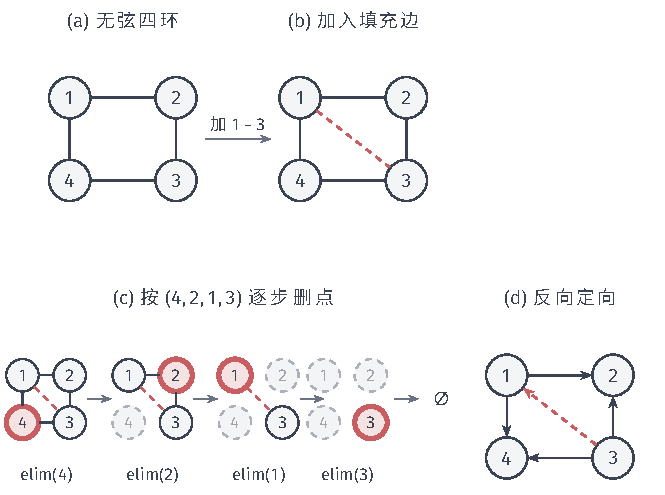
\includegraphics[width=\linewidth]{figures/03-models/03-probabilistic-graphical-models/tikz/pgm-representations-chordal-conversion/figure.pdf}
  \caption{从无弦四环到完美有向图。先加入虚线填充边$1-3$完成弦化，再按完美消除序$(4,2,1,3)$逐步删点；红色双圈标出当前消去节点，已消去节点保留为灰色虚线轮廓，便于跨快照对照。序列上方给出通用规则：$\operatorname{elim}(X_k)$时补齐其未消去邻居为团。最终从序中较晚节点指向较早节点；实线箭头来自原四环，虚线箭头来自填充边。}
  \label{fig:pgm-representations-chordal-conversion}
\end{figure}

\section{有向图与无向图的条件独立性关系}
\label{sec:pgm-representations-independence}

结构转换本身只说明怎样改图，还没有说明改图前后的概率语义是否相同。一张图通常只给出分布必须满足的一部分独立性，而不声称相连的变量一定依赖。要比较不同图，先把“图能读出什么”与“分布实际上满足什么”分别记下来，才能准确判断转换保留了哪些信息。

\subsection{独立性映射}
\label{sec:pgm-representations-maps}

记$\mathcal{I}(p)$为分布$p$实际满足的条件独立关系集合：
\begin{equation}
  \mathcal{I}(p)
  =
  \bigl\{(A,B\mid S):
  \bm{X}_A\perp\bm{X}_B\mid\bm{X}_S\bigr\},
  \label{eq:pgm-representations-distribution-independences}
\end{equation}
其中$A,B,S\subseteq V$两两不交，$A,B$非空，$S$可以为空。记$\mathcal{I}(\mathcal{G})$为图的分离规则蕴含的同类集合：有向图使用d-分离，无向图使用无向分离。这里比较的是对条件变量成立的独立性，不只是某个特定取值下偶然成立的等式。

\term{独立性映射}（independency map, I-map）表示图没有作出错误的独立性声明，但允许漏掉真实独立性；\term{依赖性映射}（dependency map, D-map）要求分布的真实独立性都能在图上找到，但允许图多声明一些。两种要求同时成立，才是\term{完美映射}（perfect map），即图与分布在独立性上完全一致。

\begin{definition}[三类独立性映射]
  \label{def:pgm-representations-maps}
  对同一组随机变量的分布$p$与图$\mathcal{G}$，有
  \begin{equation}
    \begin{aligned}
      \mathcal{G}\text{是}p\text{的I-map}
      &\iff \mathcal{I}(\mathcal{G})\subseteq\mathcal{I}(p),\\
      \mathcal{G}\text{是}p\text{的D-map}
      &\iff \mathcal{I}(p)\subseteq\mathcal{I}(\mathcal{G}),\\
      \mathcal{G}\text{是}p\text{的完美映射}
      &\iff \mathcal{I}(\mathcal{G})=\mathcal{I}(p).
    \end{aligned}
    \label{eq:pgm-representations-map-inclusions}
  \end{equation}
\end{definition}

定义~\ref{def:pgm-directed-faithfulness}中的忠实性，正是要求有向图$\mathcal{G}$成为$p$的完美映射。可靠性保证$\mathcal{G}$是$p$的I-map，忠实性再补上D-map方向。

集合方向可以用两个极端检验。完全无向图不分离任何两个非空节点集合，因而它对任意$p$都是I-map：它没有独立性声明，也就不会声明错。反过来，无边图声明所有互不相交的变量组在给定其余不交变量后仍独立，因此它对任意$p$都是D-map，但通常不是I-map。D-map中的“依赖”来自集合包含关系的逆否表述：对于给定的$A,B,S$，若图没有用$S$分离$A,B$，则D-map条件保证$\bm{X}_A$与$\bm{X}_B$在$p$中给定$\bm{X}_S$也不独立。这一要求涉及全部查询，不限于相邻节点。实际建模通常先要求I-map，因为错误地删除真实依赖，会把$p$排除在模型之外\scite{pgm-koller2009}

即使I-map中的每条边都不能再删，它也不一定是完美映射。\term{最小I-map}（minimal I-map）只要求删去任何一条边后，图不再是$p$的I-map；这里的“最小”是相对于删边操作而言，不要求在所有候选图中边数最少，也不要求唯一。以两个二元变量为例，令
\[
  p(0,0)=p(1,1)=0.4,\qquad
  p(0,1)=p(1,0)=0.1.
\]
由于$p(X_1=0)=p(X_2=0)=0.5$而$p(0,0)\ne0.25$，两变量不独立。$X_1\to X_2$和$X_1\leftarrow X_2$都是最小I-map：保留边时没有错误声明，删边就会错误地要求独立。这个例子也说明，最小性不足以确定方向。一般情况下，某张最小I-map仍可能漏掉无法由其图形同时表达的其他独立性。

同样的记号可以用于两张图的比较：若$\mathcal{I}(\mathcal{G}_2)\subseteq\mathcal{I}(\mathcal{G}_1)$，则$\mathcal{G}_2$是$\mathcal{G}_1$的I-map。此时$\mathcal{G}_2$施加的独立性约束较少；只考虑Markov约束而不另加参数限制时，它容纳的分布族较大。后面出现的道德化和填充边，主要沿着这个方向改变图。

\subsection{d-分离的无向判据}
\label{sec:pgm-representations-ancestral-moralization}

祖先图已经排除不可能参与当前查询的节点，道德图则把碰撞结构的影响转成普通无向边。于是，d-分离可以改写为祖先道德图上的无向分离。

\begin{theorem}[祖先道德化判据]
  \label{thm:pgm-representations-ancestral-moralization}
  设$\mathcal{G}=(V,E)$为有限有向无环图，$A,B,S\subseteq V$两两不交且$A,B$非空，并令
  \[
    U=\operatorname{an}^{+}(A\cup B\cup S).
  \]
  则$A$与$B$在$\mathcal{G}$中被$S$ d-分离，当且仅当它们在$\operatorname{mor}(\mathcal{G}[U])$中被$S$无向分离。
\end{theorem}

\begin{proof}[定理~\ref{thm:pgm-representations-ancestral-moralization}的证明]
先设原有向图有一条给定$S$时连接$A$与$B$的活跃路径。路径上的碰撞节点属于$\operatorname{an}^{+}(S)$。从任一非碰撞内部节点出发，至少能沿路径的一侧顺着箭头前进，直到到达端点或碰撞节点，所以该节点也是$A\cup B\cup S$中某个节点的祖先。整条路径因而位于$\mathcal{G}[U]$中。凡遇到属于$S$的碰撞片段$u\to c\leftarrow v$，就用道德图中的边$u-v$替代；非碰撞节点本来就不在$S$中。替换得到一条避开$S$的无向路线，删去重复片段便得到无向路径。

反过来，设$\operatorname{mor}(\mathcal{G}[U])$中有一条避开$S$、连接$A$与$B$的路径。保留来自原有向图骨架的边，把每条道德化新增边$u-v$展开为$u\to c\leftarrow v$，其中$c\in U$是使该边加入的共同子节点。展开后可能重复经过节点，暂称为路线。原无向路径上的节点都不在$S$中，新插入的节点在插入位置都是碰撞节点，但其中某些碰撞节点可能只属于$A$或$B$的祖先，而不属于$\operatorname{an}^{+}(S)$。

对这种尚未打开的碰撞节点$c$，若$c$本身属于$A$或$B$，就在该位置截去路线对应的前缀或后缀，使$c$成为端点。否则，由$c\in U$可知，存在从$c$到$A\cup B$中某个节点的有向路径；这条有向路径不经过$S$，否则$c$已经属于$\operatorname{an}^{+}(S)$。若终点在$A$中，就用该有向路径的反向行走替换原路线从$A$端点到$c$的部分；若终点在$B$中，则替换$c$到$B$端点的部分。新的接合处$c$有一条向外的边，因而不再是碰撞节点，替换段内部也没有碰撞节点。每次操作至少减少一个未打开的碰撞位置，且不会增加新的未打开位置，有限次后得到活跃路线。

还需从可能重复节点的活跃路线取得路径。取一条长度最短的活跃路线。若内部节点$v$出现两次，删除两次出现之间的片段；除接合处$v$外，所有节点的角色不变。若$v\in S$，两个出现位置原本都必须是碰撞位置，接合后仍是碰撞；若$v\notin S$，唯一可能出错的是接合后形成一个不属于$\operatorname{an}^{+}(S)$的碰撞节点。此时被删片段从$v$沿出边开始，又逆着$v$的另一条出边返回，沿该片段必然遇到一个作为$v$后代的碰撞节点。原路线活跃使这个碰撞节点属于$\operatorname{an}^{+}(S)$，进而推出$v\in\operatorname{an}^{+}(S)$，与可能出错的假设矛盾。端点重复时直接截去相应前缀或后缀即可。因此最短活跃路线没有重复节点，是所需的活跃路径。
\end{proof}

这个判据是纯图论结论，不依赖某张条件概率表，也不要求分布严格为正。应用时应依次确定相关祖先、取诱导子图、道德化，再删除条件节点$S$检查连通性。不能先删除条件节点再道德化，因为一个被观察的碰撞点虽将从无向查询图中删除，它的父节点之间却必须留下新增边。祖先道德图与全局Markov性质的系统论述可参见Lauritzen的教材\scite{pgm-lauritzen1996}

图~\ref{fig:pgm-representations-ancestral-moralization}展示查询$F\perp S\mid A$的转换。删除条件节点$A$以后，补出的$H-S$边仍使$F-H-S$连通，所以图不能推出该条件独立。若改为检验$F\perp S$，相关祖先只有$\{F,S\}$：$H,A,D$都不是这两个根节点的祖先，查询祖先图没有边，因而得到独立性。这一对比说明，图中原始箭头虽然固定，查询祖先图与道德化时需要补出的边却随$(A,B\mid S)$改变；图上未分离只是否定结构保证，并不声称每组参数都一定产生依赖。

保留祖先并不是保留端点的另一种说法。在辅助例子$X_1\leftarrow X_0\to X_2$中，查询$X_1\perp X_2$时，$X_0$不在端点集合中，却是必须保留的共同祖先；只保留$\{1,2\}$会错误地把两个节点分开。条件节点的祖先也不可漏掉：在$X_1\to X_3\leftarrow X_2$、$X_3\to X_4$中，给定$X_4$会激活$X_3$处的碰撞结构。查询$\{1\}$与$\{2\}$给定$\{4\}$时必须保留$X_3$，道德化才会生成$1-2$边。

这里还要区分\emph{为查询构造的祖先道德图}与\emph{整个有向图的道德图}。若把报警模型整体道德化，即使查询没有给定$A$，$F-H-S$也始终存在，原来的$F\perp S$就无法从这张无向图读出。整体道德化并非错误操作，它服务于联合因子分解的转换；只是它通常给出较弱的独立性描述。准确的图关系是
\begin{equation}
  \mathcal{I}\bigl(\operatorname{mor}(\mathcal{G})\bigr)
  \subseteq \mathcal{I}(\mathcal{G}),
  \label{eq:pgm-representations-moral-inclusion}
\end{equation}
而不是相等。整体道德图中若已经被$S$分离，在更小的祖先道德图中仍被分离，所以它可以证明一部分d-分离；整体图中连通则不能据此否定原有向图中的d-分离。

\subsection{有向图独立性结论的证明}
\label{sec:pgm-representations-directed-proofs}

祖先道德化不仅给出检测方法，也补上了第~\ref{chap:pgm-directed}章各项结论之间的证明链。下面集中给出这些证明：先处理局部归一化和分解关系，再用祖先道德图证明全局Markov性质，最后处理Markov毯与完备性；每一步只调用此前已经定义或证明的对象。

\begin{proof}[引理~\ref{lem:pgm-directed-normalization}的证明]
取有向图一个拓扑序中的最后一个节点。它没有子节点，故在全部乘积中只有自己的因子依赖它；对该节点关于$\mu_i$积分后，这个因子变成$1$。按逆拓扑序重复消去节点，由非负性和Tonelli定理可以交换积分次序，最终得到总积分$1$。有限离散情形中，这些积分就是求和。

对祖先边缘化结论，只消去$V\setminus W$。由于$W$包含其中每个节点的全部祖先，$V\setminus W$中的节点不可能有位于$W$的子节点。按照逆拓扑序消去补集时，当前节点在补集中的子节点都已经消去，因此当前剩余乘积中仍只有自己的因子依赖它。依次积分后留下且仅留下式~\eqref{eq:pgm-directed-ancestral-marginal}中的因子。
\end{proof}

\begin{proof}[定理~\ref{thm:pgm-directed-ordered-factor}的证明]
按有序Markov假设所固定的拓扑序应用概率链式法则：
\[
  p(x_1,\ldots,x_d)=
  \prod_{i=1}^{d}p(x_i\mid x_1,\ldots,x_{i-1}).
\]
由式~\eqref{eq:pgm-directed-ordered}，每个条件项都可以删除非父前驱变量，即
\[
  p(x_i\mid\bm{x}_{\operatorname{pre}(i)})
    =p(x_i\mid\bm{x}_{\operatorname{pa}(i)}).
\]
将这些等式代回链式法则，便得到式~\eqref{eq:pgm-directed-factorization}。条件等式在对应前驱配置的分布下几乎处处成立。离散情形若某个前缀具有零概率，后续条件表可以任意归一化补全，因为该前缀对应的联合概率仍为零；也可以按前缀长度归纳验证两个乘积给出的前缀分布始终相同。连续情形使用条件密度的版本，得到几乎处处相同的联合密度。整个证明始终使用同一个拓扑序。
\end{proof}

\begin{proof}[定理~\ref{thm:pgm-directed-factor-local}的证明]
固定节点$i$，令$N=\operatorname{nd}(i)$。$N$中的节点既不可能以$i$为祖先，也不可能以$i$的后代为祖先；$i$的祖先又都属于$N$。因此，$N$与$N\cup\{i\}$都包含其中每个节点的全部祖先。由引理~\ref{lem:pgm-directed-normalization}的祖先边缘化结论，
\[
  \begin{aligned}
    p(x_i,\bm{x}_N)
      &=q_i(x_i\mid\bm{x}_{\operatorname{pa}(i)})
        \prod_{j\in N}q_j(x_j\mid\bm{x}_{\operatorname{pa}(j)})\\
      &=q_i(x_i\mid\bm{x}_{\operatorname{pa}(i)})p(\bm{x}_N).
  \end{aligned}
\]
于是$p(x_i\mid\bm{x}_N)=q_i(x_i\mid\bm{x}_{\operatorname{pa}(i)})$，等式按条件分布的定义域理解。再对$N\setminus\operatorname{pa}(i)$边缘化，可知$q_i$也是$p(x_i\mid\bm{x}_{\operatorname{pa}(i)})$的一个版本；条件分布不依赖非父节点的非后代，局部Markov性质成立。

在任一固定拓扑序中，$\operatorname{pre}(i)\subseteq N$。从局部独立陈述中边缘化其余非后代，便得到该顺序下的有序Markov性质。这里是在局部性质成立以后使用集合包含关系，没有预先假设分布满足另一个顺序的有序性质。
\end{proof}

接下来证明全局结论。以下用求和写离散情形；对于具有联合密度的连续变量，将求和换成相对于相应基准测度的积分，并用Tonelli定理交换非负函数的积分次序。

\begin{proof}[定理~\ref{thm:pgm-directed-soundness}的证明]
设$p\in\mathcal{M}(\mathcal{G})$且$A\perp_{\mathcal{G}}B\mid S$。由定理~\ref{thm:pgm-directed-ordered-factor}，$p$按$\mathcal{G}$分解，记节点$i$的局部因子为$q_i(x_i\mid\bm{x}_{\operatorname{pa}(i)})$。令$R=\operatorname{an}^{+}(A\cup B\cup S)$，对$V\setminus R$边缘化后，由引理~\ref{lem:pgm-directed-normalization}，
\[
  p(\bm{x}_R)=
  \prod_{i\in R}q_i(x_i\mid\bm{x}_{\operatorname{pa}(i)}).
\]
每个因子的作用域$\{i\}\cup\operatorname{pa}(i)$在$\operatorname{mor}(\mathcal{G}[R])$中两两相连。删去$S$后，一个因子的非条件节点不可能分属两个连通分量，否则这些节点之间的无向边会连接相应分量。

令$C$为$\operatorname{mor}(\mathcal{G}[R])\setminus S$中所有与$A$相交的连通分量之并，令$D=R\setminus(C\cup S)$。由定理~\ref{thm:pgm-representations-ancestral-moralization}，$B\subseteq D$。把非条件作用域落在$C$中的因子相乘得到$g(\bm{x}_C,\bm{x}_S)$，落在$D$中的因子相乘得到$h(\bm{x}_D,\bm{x}_S)$，只涉及$S$的因子相乘得到$k(\bm{x}_S)$，于是
\[
  p(\bm{x}_R)=
  g(\bm{x}_C,\bm{x}_S)
  h(\bm{x}_D,\bm{x}_S)
  k(\bm{x}_S).
\]
分别对$C\setminus A$和$D\setminus B$边缘化，记所得函数为$g_A,h_B$，便有
\[
  p(\bm{x}_A,\bm{x}_B,\bm{x}_S)=
  g_A(\bm{x}_A,\bm{x}_S)
  h_B(\bm{x}_B,\bm{x}_S)
  k(\bm{x}_S).
\]
对具有正且有限边缘质量或密度的$\bm{x}_S$，令$G(\bm{x}_S)=\sum_{\bm{x}_A}g_A(\bm{x}_A,\bm{x}_S)$、$H(\bm{x}_S)=\sum_{\bm{x}_B}h_B(\bm{x}_B,\bm{x}_S)$。对条件联合分布归一化后，
\[
  \begin{aligned}
    p(\bm{x}_A,\bm{x}_B\mid\bm{x}_S)
      &=\frac{g_A(\bm{x}_A,\bm{x}_S)}{G(\bm{x}_S)}
        \frac{h_B(\bm{x}_B,\bm{x}_S)}{H(\bm{x}_S)}\\
      &=p(\bm{x}_A\mid\bm{x}_S)
        p(\bm{x}_B\mid\bm{x}_S).
  \end{aligned}
\]
零质量条件值无需作比值，连续密度中的异常取值按几乎处处约定处理。由此得到所需条件独立性，且证明不要求联合分布严格为正。
\end{proof}

\begin{proof}[定理~\ref{thm:pgm-directed-markov-blanket}的证明]
令$O=V\setminus(\{i\}\cup\operatorname{mb}(i))$。若$O=\varnothing$，则定理所述的条件独立按定义平凡成立。以下设$O\neq\varnothing$，并考虑任意一条从$i$到$O$中节点的路径。路径的第一个相邻节点不可能已经属于$O$，因为$i$的每个父节点和子节点都在$\operatorname{mb}(i)$中。

若路径先经过父节点$j\to i$，则$j$在路径上是非碰撞节点，而且$j\in\operatorname{mb}(i)$，所以给定Markov毯会在$j$处阻断路径。若路径先沿$i\to j$经过子节点$j$，随后沿$j\to k$离开，则$j$是已给定的非碰撞节点，路径同样被阻断。剩下的情形是路径以$i\to j\leftarrow k$开头；此时$j$虽是已给定的碰撞节点，但$k$是$j$的另一个父节点，因而也属于$\operatorname{mb}(i)$。节点$k$不是路径终点，并且边$k\to j$在$k$处给出箭尾，所以$k$是已给定的非碰撞节点，路径在此被阻断。

所有从$i$到$O$的路径都被$\operatorname{mb}(i)$阻断，即$i\perp_{\mathcal G}O\mid\operatorname{mb}(i)$。定理~\ref{thm:pgm-directed-soundness}再把这个图论分离转成定理所述的条件独立。

同一屏蔽关系也可以从局部因子直接读出。由定理~\ref{thm:pgm-directed-ordered-factor}，给定其余变量后，联合乘积中只有节点$i$及其子节点的因子含$x_i$，所以
\begin{equation}
  \begin{aligned}
    p(x_i\mid\bm{x}_{V\setminus\{i\}})
      &\propto q_i(x_i\mid\bm{x}_{\operatorname{pa}(i)})\\
      &\quad{}\times
      \prod_{j\in\operatorname{ch}(i)}
        q_j(x_j\mid\bm{x}_{\operatorname{pa}(j)}).
  \end{aligned}
  \label{eq:pgm-directed-blanket-conditional}
\end{equation}
右侧除$x_i$外只涉及$\operatorname{mb}(i)$中的变量，对$x_i$归一化不会引入毯外变量。比例式只在条件分布有定义的配置上使用；零概率条件配置仍按第~\ref{chap:pgm-directed}章约定选取条件分布版本。
\end{proof}

现在可以闭合第~\ref{chap:pgm-directed}章的四种表述。有序Markov性质由定理~\ref{thm:pgm-directed-ordered-factor}推出因子分解；因子分解由定理~\ref{thm:pgm-directed-soundness}推出全局Markov性质；全局性质由引理~\ref{lem:pgm-representations-global-to-local}推出局部性质；局部性质又由定理~\ref{thm:pgm-directed-factor-local}中的边缘化论证推出任一拓扑序下的有序性质。因此式~\eqref{eq:pgm-directed-equivalence}成立，并且整个等价链不要求联合分布严格为正。

完备性处理相反方向：若图中仍有活跃路径，需要证明至少能选择一组相容参数，使路径两端在给定条件集后确实不独立。先看一个可以逐项复算的连续构造。考虑图$X\to Z\leftarrow Y$以及$Z\to D$，令
\[
  \begin{aligned}
    X&=\varepsilon_X,& Y&=\varepsilon_Y,\\
    Z&=X+Y+\varepsilon_Z,& D&=Z+\varepsilon_D,
  \end{aligned}
\]
其中四个噪声相互独立，均服从$\mathcal{N}(0,1)$。该分布按有向图分解，且$X,Y$边缘独立。由高斯条件协方差公式，
\[
  \begin{aligned}
    \operatorname{Cov}(X,Y\mid Z)
      &=0-\frac{1\cdot1}{3}=-\frac13,\\
    \operatorname{Cov}(X,Y\mid D)
      &=0-\frac{1\cdot1}{4}=-\frac14.
  \end{aligned}
\]
条件协方差公式来自将每个变量对观测作线性回归后，计算两个回归残差的协方差；对联合高斯变量，残差与观测独立，故它正是条件协方差。两个非零结果分别验证了观测碰撞节点、观测其后代时的依赖，但这个四节点构造还不能代替任意有向图上的证明。

一般图中的活跃路径可能包含多个碰撞节点，它们通向条件节点的有向路径还可能相交。直接声称“给活跃路径每条边一个非零系数就必然不独立”并不成立。图~\ref{fig:pgm-directed-cancellation}给出反例：令
\[
  X=\varepsilon_X,\qquad
  Z=X+\varepsilon_Z,\qquad
  Y=-X+Z+\varepsilon_Y,
\]
各噪声仍相互独立且服从$\mathcal N(0,1)$。图中三条边的系数都非零，但代入后$Y=\varepsilon_Z+\varepsilon_Y$，从而$X\perp Y$。直接路径与间接路径的作用恰好抵消。改变$X\to Y$的系数为$-1+\delta$，则$\operatorname{Cov}(X,Y)=\delta$；只要$\delta\ne0$，这个额外独立性便消失。

\begin{figure}[htbp]
  \centering
  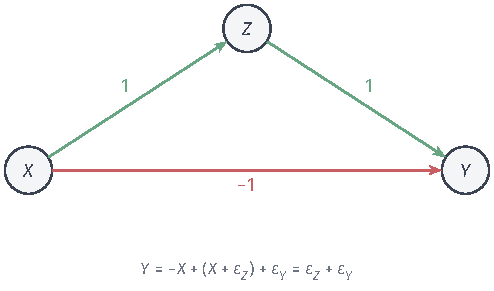
\includegraphics[width=\linewidth]{figures/03-models/03-probabilistic-graphical-models/tikz/pgm-directed-cancellation/figure.pdf}
  \caption{参数抵消造成的额外独立性。$X\to Y$的直接系数为$-1$，经$Z$的两条系数均为$1$；两条路径都没有被空集阻断，但这个特定高斯分布中$X$与$Y$独立。}
  \label{fig:pgm-directed-cancellation}
\end{figure}

一般有向图上的完备性依赖下面的关键引理。它的作用是排除“所有相容参数都因路径抵消而满足额外独立性”的可能；后面的代数论证只负责从非零多项式得到所需参数，不会把这一关键图论事实重新证明。离散结论及其路径构造见Meek的强完备性证明，高斯结论可由线性高斯有向图的标准多项式完备性论证得到\scite{pgm-directed-meek1995,pgm-koller2009}

\begin{lemma}[条件独立约束的非平凡性]
  \label{lem:pgm-directed-nontrivial}
  设$\mathcal{G}=(V,E)$为有限有向无环图，$u,v\in V$为不同节点，$S\subseteq V\setminus\{u,v\}$，且$u,v$在$\mathcal{G}$中给定$S$时d-连接，则以下两项成立。
  \begin{enumerate}
    \item 对$i\in V$，在线性高斯系统
    \[
      X_i=\sum_{j\in\operatorname{pa}(i)}b_{i,j}X_j+\varepsilon_i,
      \qquad
      \varepsilon_1,\ldots,\varepsilon_d
      \mathrel{\overset{\mathrm{ind}}{\sim}}\mathcal N(0,1)
    \]
    中，记边系数为$\bm{\theta}$、协方差矩阵为$\bm{\Sigma}(\bm{\theta})$，则
    \[
      f_{u,v,S}(\bm{\theta})
      =\det\bm{\Sigma}_{(u,S),(v,S)}(\bm{\theta})
    \]
    是非零多项式。行指标按$u$及$S$排列，列指标按$v$及同一顺序的$S$排列；$S=\varnothing$时，该式为$\Sigma_{u,v}$。
    \item 固定每个节点至少含两个状态的有限状态空间，并用各行前$r_i-1$个概率参数化局部条件表。将联合概率与边缘概率写成这些参数的多项式后，在所有状态配置对应的条件独立多项式
    \[
      p(x_u,x_v,\bm{x}_S)p(\bm{x}_S)
      -p(x_u,\bm{x}_S)p(x_v,\bm{x}_S)
    \]
    中，至少有一个不是零多项式。
  \end{enumerate}
\end{lemma}

这项引理在此作为有来源的外部结果使用，不把路径缩减的说明冒充完整证明。其证明需要从活跃路径及碰撞节点通向$S$的有向路径中提取仍保留连接的子图，并控制这些路径交会时可能发生的代数抵消。高斯模型允许任意正噪声方差；单位方差子类已经足以证明存在性，而逐坐标可逆缩放也不改变条件独立性。

\begin{proof}[定理~\ref{thm:pgm-directed-completeness}的线性高斯部分]
若集合$A,B$未被$S$ d-分离，就有某个$u\in A,v\in B$之间存在活跃路径。在引理~\ref{lem:pgm-directed-nontrivial}的线性系统中，令$\bm{B}$为严格下三角系数矩阵，其非边元素为零。因为$\bm{B}^d=\bm 0$，
\[
  \begin{aligned}
    \bm{L}&=(\bm{I}-\bm{B})^{-1}
       =\bm{I}+\bm{B}+\cdots+\bm{B}^{d-1},\\
    \bm{\Sigma}(\bm{\theta})&=\bm{L}\bm{L}^{\top}.
  \end{aligned}
\]
因此协方差的每个元素都是边系数的多项式，且对所有实边系数，$\bm{\Sigma}$都正定。分块行列式恒等式给出
\[
  f_{u,v,S}(\bm{\theta})
    =\det(\bm{\Sigma}_{S,S})
      \bigl(\Sigma_{u,v}
        -\bm{\Sigma}_{u,S}\bm{\Sigma}_{S,S}^{-1}
         \bm{\Sigma}_{S,v}\bigr).
\]
括号内是$\operatorname{Cov}(X_u,X_v\mid\bm X_S)$；$S$为空时约定空矩阵行列式为$1$，不执行矩阵求逆。高斯条件分布中，这个协方差为零当且仅当两个标量条件独立。引理说明$f_{u,v,S}$不是零多项式，因而存在系数使它不为零。

还可以给出一个不追求效率的确定构造：按有理数分子绝对值和正分母的界依次枚举所有有理边系数向量，逐一用有理数运算计算上述行列式，找到非零值就停止。非零多项式在某个实参数点附近保持非零，而有理向量在实空间中稠密，所以枚举必会停止。输出系数与单位独立高斯噪声定义一个属于$\mathcal{M}_{\mathrm{LG}}(\mathcal{G})$的分布，且$X_u\not\perp X_v\mid\bm X_S$。若整个向量$\bm X_A,\bm X_B$条件独立，其任意坐标对也应条件独立，与这个结果矛盾；所求集合查询的反例由此构造出来。
\end{proof}

有限离散变量不能用高斯构造代替。将每张局部条件概率表中除最后一个状态以外的概率作为自由参数，最后一个概率由行和为$1$确定；严格正条件表构成这个有限维参数空间中的一个非空开集。联合概率和边缘概率都是这些参数的多项式，而给定$S$时$X_u$与$X_v$条件独立，等价于对所有状态配置同时满足
\[
  \begin{aligned}
    &p(x_u,x_v,\bm x_S)p(\bm x_S)\\
    &\qquad{}-p(x_u,\bm x_S)p(x_v,\bm x_S)=0.
  \end{aligned}
\]

\begin{proof}[定理~\ref{thm:pgm-directed-completeness}的有限离散部分]
仍取活跃路径连接的$u\in A,v\in B$。引理~\ref{lem:pgm-directed-nontrivial}的第二项表明，上述有限组多项式中至少有一个不是零多项式。非零多项式不可能在参数空间的非空开集上处处为零，因此存在一组严格为正的局部条件表，使至少一个条件独立等式失败。由这些条件表得到的联合分布属于$\mathcal{M}_{\mathrm{disc}}^{+}(\mathcal{G})$，且$X_u\not\perp X_v\mid\bm X_S$。若$\bm X_A\perp\bm X_B\mid\bm X_S$成立，则任意坐标对也应条件独立，产生矛盾。因此$\bm X_A\not\perp\bm X_B\mid\bm X_S$。
\end{proof}

同一多项式论证还解释了忠实分布为何存在。在固定有限图上，需要检查的节点对与条件集合只有有限多组；每个未分离查询出现额外独立性，都要求相应的一个或多个非零多项式同时取零。非零多项式的零点集具有Lebesgue测度零，有限个零点集之并仍不能覆盖具有非空内部的参数空间。因此，在上述不受额外限制的离散或线性高斯参数族中存在忠实分布，而且不忠实参数只占零测集。这个结论不保证真实系统必然忠实，也不排除参数接近抵消集合时，有限样本很难识别微弱依赖。

\subsection{两类独立性表示的差异}
\label{sec:pgm-representations-independence-differences}

祖先道德化借助“每个查询一张图”复现d-分离，并没有给出一张同时回答全部查询的完美无向图。这个区别在最小的碰撞结构$X_1\to X_3\leftarrow X_2$中已经出现：有向图声明$X_1\perp X_2$，却不声明$X_1\perp X_2\mid X_3$。在任何无向图中，若$1$与$2$已被空集分离，它们原本就没有路径；再删除节点$3$不可能创造路径。因而同一节点集合上不存在具有完全相同分离关系的无向图。这里否定的是图独立性集合的完全相同，不是某个特殊分布碰巧可由两类图共同表示。

无向图也有有向图不能完美表达的结构。考虑图~\ref{fig:pgm-representations-chordal-conversion}左侧的四环$1-2-3-4-1$，其中没有$1-3$或$2-4$边。它同时声明
\begin{equation}
  X_1\perp X_3\mid(X_2,X_4),\qquad
  X_2\perp X_4\mid(X_1,X_3).
  \label{eq:pgm-representations-cycle-independences}
\end{equation}
若要用同一骨架定向，又不形成有向环，就必须使某个环上节点同时接收两条邻边。例如令$2\to1\leftarrow4$，由于$2$与$4$不相邻，便出现了未被邻接边遮蔽的碰撞结构。给定$\{1,3\}$反而会打开$2\to1\leftarrow4$，与式~\eqref{eq:pgm-representations-cycle-independences}中的第二个独立性冲突。

为什么必须出现这种碰撞？取任意拓扑序，选择四环中排在最晚的节点，其两个环上邻居都排在它之前，邻边便都指向它。更换拓扑序只能移动碰撞的位置，不能消除这个问题。具有相同独立性的有向图也不能通过改变骨架来避开反例。具体地说，对有向图中任意两个不相邻节点$i,j$，无环性保证至少可以选择其中一个节点，例如$i$，使$j$不是$i$的后代。由于$j$也不是$i$的父节点，局部Markov性质给出某个分离关系，例如$X_i\perp X_j\mid\bm{X}_{\operatorname{pa}(i)}$。无向图中的不相邻节点则可由其余所有节点分离。反过来，无论在有向图还是无向图中，相邻节点之间长度为一的路径都不可能被不含端点的条件集阻断。因此，一张图的全部分离关系能够确定哪些节点相邻；两张图若有相同的独立性集合，骨架就必须相同。

碰撞结构与无弦四环分别给出一种无法跨图类型完美表达的独立性模式，说明两类表示的一般表达能力互不包含。不过，这些反例不意味着任何有向图和无向图都无法对应；第~\ref{sec:pgm-representations-chordal-conversion}节定义的弦图与完美有向图恰好刻画了可以完美转换的边界。

\subsection{完美表示的条件}
\label{sec:pgm-representations-perfect-dags}

有限无向图是弦图，当且仅当它存在完美消除序。下面借助这一标准图论结果，分别陈述无向图何时有完美有向表示、有向图何时有完美无向表示；弦图与消除序等价性的图论证明可参见分解图的相关论述\scite{pgm-lauritzen1996}

\begin{theorem}[无向图的完美有向图表示]
  \label{thm:pgm-representations-chordal-perfect}
  设$\mathcal{U}=(V,E_{\mathcal U})$为有限无向图。存在以同一有限节点集合$V$为节点集的有向无环图$\mathcal{D}=(V,E_{\mathcal D})$，使按无向分离定义的$\mathcal{I}(\mathcal{U})$与按d-分离定义的$\mathcal{I}(\mathcal{D})$满足
  \[
    \mathcal{I}(\mathcal{D})=\mathcal{I}(\mathcal{U}),
  \]
  当且仅当$\mathcal{U}$是弦图。若$v_1,\ldots,v_d$是$\mathcal{U}$的完美消除序，将每条边从序中较晚的节点指向较早的节点，便得到一个满足上述等式的完美有向图$\mathcal{D}$。
\end{theorem}

\begin{proof}
按上述规则定向时，沿箭头移动会使序号严格减小，因此$\mathcal{D}$没有有向环。$v_k$的父集恰好是$N_k^+$，由完美消除序的定义可知其中的节点两两相邻，空父集也满足要求。

为证明独立性集合相同，先设$\mathcal{U}$中存在一条避开$S$、连接$A$与$B$的路径，并选取最短的一条。若它在$\mathcal{D}$中有碰撞点，则该点两侧节点都是其父节点，必然有边直接相连。用这条边可以缩短路径，产生矛盾。因此这条最短路径没有碰撞点，又没有经过$S$，故在$\mathcal{D}$中活跃。反过来，若$\mathcal{D}$中存在活跃路径，则其中属于$S$的节点只能是碰撞点。利用这些碰撞点父节点间已有的边逐一绕过它们，就得到一条避开$S$的无向行走；去掉重复片段即可得到$\mathcal{U}$中的无向路径。这证明两种分离判断对每个$(A,B\mid S)$都等价。

为证明必要性，假设存在满足独立性集合相等的有限有向无环图$\mathcal{D}$。由前述邻接判据，$\operatorname{skel}(\mathcal{D})=\mathcal{U}$。$\mathcal{D}$不能含有未被遮蔽的碰撞$i\to k\leftarrow j$：不相邻的$i,j$中至少有一个不是另一个的后代，取相应节点的父集便得到一个不含共同子节点$k$的d-分离集；无向路径$i-k-j$却不会被这个集合阻断，与独立性集合相等矛盾。若$\mathcal{U}$含有长度至少为四的诱导环，取该环中在$\mathcal{D}$的拓扑序里最晚的节点，其两个环上邻居都会指向它，而且两邻居在诱导环中不相邻，从而形成未被遮蔽的碰撞。故$\mathcal{U}$必须是弦图。
\end{proof}

\Needspace{14\baselineskip}
\begin{theorem}[有向图的完美无向图表示]
  \label{thm:pgm-representations-perfect-undirected}
  设$\mathcal{D}=(V,E_{\mathcal D})$为有限有向无环图。存在以同一有限节点集合$V$为节点集的有限无向图$\mathcal{U}=(V,E_{\mathcal U})$，使按d-分离定义的$\mathcal{I}(\mathcal{D})$与按无向分离定义的$\mathcal{I}(\mathcal{U})$满足
  \[
    \mathcal{I}(\mathcal{U})=\mathcal{I}(\mathcal{D}),
  \]
  当且仅当$\mathcal{D}$是完美有向图。条件成立时，$\operatorname{skel}(\mathcal{D})$是弦图，并且可以取$\mathcal{U}=\operatorname{skel}(\mathcal{D})$。
\end{theorem}

\begin{proof}
先设$\mathcal{D}$是完美有向图，并取它的任一拓扑序$t_1,\ldots,t_d$。逆序$t_d,\ldots,t_1$是$\operatorname{skel}(\mathcal{D})$的完美消除序：删除$t_i$时尚未删除的邻居恰好是$t_i$的父节点，而这些父节点按完美有向图的定义已经成团。因此$\operatorname{skel}(\mathcal{D})$是弦图；沿该完美消除序从较晚节点向较早节点定向，恰好恢复原图$\mathcal{D}$。由定理~\ref{thm:pgm-representations-chordal-perfect}，
\[
  \mathcal{I}\bigl(\operatorname{skel}(\mathcal{D})\bigr)
  =\mathcal{I}(\mathcal{D}),
\]
所以取$\mathcal{U}=\operatorname{skel}(\mathcal{D})$即可。

反过来，设存在同一节点集合上的有限无向图$\mathcal{U}$满足$\mathcal{I}(\mathcal{U})=\mathcal{I}(\mathcal{D})$。邻接判据给出$\mathcal{U}=\operatorname{skel}(\mathcal{D})$。若$\mathcal{D}$含有未被遮蔽的碰撞$i\to k\leftarrow j$，则$i,j$不相邻。两者中至少有一个不是另一个的后代，不妨设$j$不是$i$的后代；于是$i$与$j$在$\mathcal{D}$中被$\operatorname{pa}(i)$ d-分离，而且作为$i$的子节点，$k\notin\operatorname{pa}(i)$。无向图$\mathcal{U}$中的路径$i-k-j$仍然避开$\operatorname{pa}(i)$，所以同一条件集不能无向分离$i,j$，产生矛盾。因此$\mathcal{D}$不含未被遮蔽的碰撞，也就是完美有向图。
\end{proof}

此处“完美有向图”描述父集成团这一图结构性质；“$\mathcal{D}$是$p$的完美映射”还涉及具体分布。即使$\mathcal{D}$与$\mathcal{U}$的图独立性完全相同，某组特殊参数仍可能使$p$多出额外独立性，不能混淆这两个“完美”。

图~\ref{fig:pgm-representations-chordal-conversion}也展示了不满足条件时怎样放宽结构。对四环加入$1-3$，得到两个极大团$\{1,2,3\}$和$\{1,3,4\}$；若原图为$\mathcal{U}$、弦化后为$\widetilde{\mathcal{U}}$，则
\[
  \mathcal{I}(\widetilde{\mathcal{U}})
  \subseteq \mathcal{I}(\mathcal{U}).
\]
因为填充边只能增加路径，不会创造新的分离。四环中$X_2\perp X_4\mid(X_1,X_3)$仍可读出，但$X_1\perp X_3\mid(X_2,X_4)$不再由新图声明。弦化因此能够为消除和定向建立所需结构，代价是新图可能不再声明原图的全部独立性。

\section{有向图与无向图的因子分解关系}
\label{sec:pgm-representations-factorizations}

图独立性无法无损互换，并不意味着概率值也必须改变。若只是把同一组函数重新组织，原分布可以完整保留。这里应固定一个已给定的$p$来研究代数转换，再单独考察转换后图结构允许的更大模型族。

\subsection{两类因子分解的差异}
\label{sec:pgm-representations-normalization}

有向图模型给出
\begin{equation}
  p(\bm{x})=\prod_{i\in V}
  p(x_i\mid\bm{x}_{\operatorname{pa}(i)}).
  \label{eq:pgm-representations-directed-product}
\end{equation}
其中每张局部条件表对每种父节点配置都满足$\sum_{x_i}p(x_i\mid\bm{x}_{\operatorname{pa}(i)})=1$。这种局部归一化为什么足以保证联合归一化？取一个没有子节点的节点，它只出现在自己的条件因子中，对它求和后这个因子变为$1$。删除该节点后仍是有向图，可以重复这一过程，直到所有因子都被消去，得到$\sum_{\bm{x}}p(\bm{x})=1$。没有有向环保证了每步都能找到这样的节点。

Markov网络则以非负势函数表示
\begin{equation}
  p(\bm{x})=\frac{1}{Z}
  \prod_{C\in\mathcal{C}}\psi_C(\bm{x}_C),
  \qquad
  Z=\sum_{\bm{x}}\prod_{C\in\mathcal{C}}\psi_C(\bm{x}_C),
  \label{eq:pgm-representations-undirected-product}
\end{equation}
其中$\mathcal{C}$是选定的团作用域集合，未必只包含极大团，并要求$0<Z<\infty$。势函数的数值是对局部配置的相对权重，不要求对任何一个变量求和为$1$。共享变量使不同势函数的归一化互相影响，所以不能把每个势单独除以其元素和，就认为联合函数已归一化。把某个势乘以正的常数会同时缩放$Z$，却不改变$p$，这也表明原始势表通常有冗余参数。

对于连续变量，应将求和改为相对于指定乘积测度的积分，并要求所得函数可测、非负且可归一化；局部密度的归一化也按相应积分理解。由给定非负团因子分解推出无向全局Markov性质，不需要额外假设严格正性；反过来，仅凭无向Markov独立性保证团分解时，严格正性等条件不能省略。本节后面的条件表重组在有限离散、严格正的分布下推导，避免在零概率条件事件上除以零。

\subsection{从有向因子分解到无向因子分解}
\label{sec:pgm-representations-directed-to-undirected}

式~\eqref{eq:pgm-representations-directed-product}中的每个因子作用于$\{i\}\cup\operatorname{pa}(i)$。在有向图的整体道德图中，这个集合恰好被连成团。因此可以直接令
\[
  \psi_{\{i\}\cup\operatorname{pa}(i)}
  (x_i,\bm{x}_{\operatorname{pa}(i)})
  =
  p(x_i\mid\bm{x}_{\operatorname{pa}(i)}),
\]
把所有这些局部因子相乘；作用域重复时，可以保留多个因子，也可以合并。乘积没有改变，原有局部归一化保证这里的$Z=1$。若希望每个极大团只有一个势，则把每个因子恰好分配给一个包含其作用域的极大团，再在团内相乘；没有分到因子的团取恒为$1$的势。这仍不改变联合函数。这里要求“极大”而非“最大”：不能再扩张的团足以覆盖全部因子，节点数最多的团却未必覆盖其他作用域。

在报警模型中，该变换为
\begin{equation}
  \begin{aligned}
    p(f,h,a,s)&=p(f)p(s)p(h\mid f)p(a\mid h,s)\\
    &=\psi_{\{F,H\}}(f,h)\,
      \psi_{\{H,A,S\}}(h,a,s),\\
    \psi_{\{F,H\}}(f,h)&=p(f)p(h\mid f),\\
    \psi_{\{H,A,S\}}(h,a,s)&=p(s)p(a\mid h,s).
  \end{aligned}
  \label{eq:pgm-representations-alarm-potentials}
\end{equation}
道德图新增了$H-S$边，团势能容纳原分布，却不再从图结构声明$F\perp S$。分布中的独立性并没有消失：对$a,h$求和仍得
\[
  \sum_h\sum_a p(f)p(s)p(h\mid f)p(a\mid h,s)
  =p(f)p(s).
\]
消失的是仅靠新图就能识别该等式的能力；它现在依赖势函数所保留的特殊归一化关系。若任意调整这两张势表而不维持这些关系，新图允许的新分布就未必仍满足$F\perp S$。

用同一组人工教学参数可以看清条件化的影响。令$p(F=1)=0.1$、$p(S=1)=0.05$，且$p(H=1\mid F=1)=0.8$、$p(H=1\mid F=0)=0.1$，则$p(H=1)=0.17$。按$(h,s)=(0,0),(1,0),(0,1),(1,1)$的顺序，设$p(A=1\mid h,s)$分别为$0.01,0.9,0.7,0.99$。这些数值不是设备实测统计。由$H$与$S$边缘独立可得
\[
  \begin{aligned}
    p(A=1)
    &=0.83\times0.95\times0.01
      +0.17\times0.95\times0.9\\
    &\quad+0.83\times0.05\times0.7
      +0.17\times0.05\times0.99\\
    &=0.1907.
  \end{aligned}
\]
给定报警之后，传感器状态会改变过热的后验概率：
\begin{equation}
  \begin{aligned}
    p(H=1\mid A=1,S=0)
    &=\frac{0.17\times0.9}
    {0.17\times0.9+0.83\times0.01}
    \approx0.9485,\\
    p(H=1\mid A=1,S=1)
    &=\frac{0.17\times0.99}
    {0.17\times0.99+0.83\times0.7}
    \approx0.2246.
  \end{aligned}
  \label{eq:pgm-representations-alarm-posteriors}
\end{equation}
这组参数确实产生了碰撞点条件化后的依赖。无论使用原有向乘积，还是式~\eqref{eq:pgm-representations-alarm-potentials}的团势乘积，计算结果都完全相同。新增$H-S$边只是使无向表示能容纳这种相互作用，不表示转换凭空改变了物理关系。

道德化还会改变图的团结构。一个有$k$个父节点的子节点，在道德图中与父节点构成$k+1$元团；父节点之间可能新增至多$\binom{k}{2}$条边。若各变量有$r$种状态，任意稠密$(k+1)$元表有$r^{k+1}$个表项。不过，这不一定是转换新带来的存储量，因为一般的原条件概率表本来就有同样大小的作用域。多个局部作用域叠加后，道德图的最大团还可能大于单个节点的家庭；将小因子过早合并成一般的极大团势表，会丢掉可利用的细分结构。

推断的实际代价取决于消除过程中形成的最大联合因子，而不只取决于输入图中边的数量。道德图也未必是弦图，后续消除可能继续引入填充边。因而道德化应被理解为获得一个容纳所有因子作用域的无向结构，不应被理解为已经找到代价最小的推断结构。

\subsection{从无向因子分解到有向因子分解}
\label{sec:pgm-representations-undirected-to-directed}

任意联合分布都能用概率链式法则沿某个顺序写成条件分布乘积，但每个条件分布可能需要之前的全部变量。这只能保证存在一个稠密有向图。若希望父集仍由原无向图的邻居给出，弦图与完美消除序才提供了所需条件。

设$p$严格为正并已在弦图$\mathcal{U}$上分解，选择完美消除序$v_1,\ldots,v_d$。下面的构造依赖一个作用域不变量：在处理$v_k$之前，每个当前因子的作用域都是剩余诱导图$\mathcal{U}[\{v_k,\ldots,v_d\}]$中的团。初始因子本来就定义在$\mathcal{U}$的团上，因此第$1$步满足该不变量。若第$k$步开始时不变量成立，那么任何含$v_k$的当前因子，除$v_k$外只能涉及其尚未删除的邻居，因而其余作用域包含在$N_k^+$中。将这些因子相乘并消去$v_k$后，新因子的作用域包含在$N_k^+$中；完美消除序保证$N_k^+$已经成团，所以新因子在下一张剩余图中仍是团因子。不含$v_k$的因子保持不变，归纳便可继续。

在第$k$步，将当前含$v_k$的因子收集到集合$\mathcal{B}_k$。由上述不变量，它们的乘积只可能依赖$v_k$及$N_k^+$中的变量。先把这些因子相乘，再对$v_k$求和：
\begin{equation}
  \begin{aligned}
    b_k(x_{v_k},\bm{x}_{N_k^+})
    &=\prod_{\psi\in\mathcal{B}_k}\psi,\\
    a_k(\bm{x}_{N_k^+})
    &=\sum_{x_{v_k}}b_k(x_{v_k},\bm{x}_{N_k^+}),\\
    q_k(x_{v_k}\mid\bm{x}_{N_k^+})
    &=\frac{b_k(x_{v_k},\bm{x}_{N_k^+})}
    {a_k(\bm{x}_{N_k^+})}.
  \end{aligned}
  \label{eq:pgm-representations-bucket-normalization}
\end{equation}
这里允许函数实际依赖的变量少于所列作用域。把$\mathcal{B}_k$中的因子从当前乘积移除，换入$a_k$，就完成了对$v_k$的边缘化。上述归纳同时说明，新的因子$a_k$不会要求原图之外的边。

$q_k$为什么是正确的条件分布，而不仅是一张随手归一化的表？消除$v_1,\ldots,v_{k-1}$后，当前乘积正比于剩余变量的联合边缘分布。除$\mathcal{B}_k$外的因子不含$v_k$，在给定其余剩余变量、对$v_k$归一化时都可约掉。因此$q_k$等于这个边缘分布中$v_k$给定所有剩余变量的条件分布，而式~\eqref{eq:pgm-representations-bucket-normalization}表明它实际上只需要$N_k^+$。这一步利用了消除产生的当前因子，不能只归一化输入时某张原始团势。

每一步都有$b_k=q_k a_k$。把这些恒等式逐层代回，末尾消除所有变量所留下的常数就是$Z$，故
\begin{equation}
  \begin{aligned}
    \prod_{C\in\mathcal{C}}\psi_C(\bm{x}_C)
    &=Z\prod_{k=1}^d q_k(x_{v_k}\mid\bm{x}_{N_k^+}),\\
    p(\bm{x})&=\prod_{k=1}^d q_k(x_{v_k}\mid\bm{x}_{N_k^+}).
  \end{aligned}
  \label{eq:pgm-representations-telescoping-product}
\end{equation}
以$N_k^+$为$v_k$的父集，就得到定理~\ref{thm:pgm-representations-chordal-perfect}中的有向图。它的拓扑序是消除序的逆序，这两个顺序不可混用。转换后的局部条件表已经归一化，但求出这些表的过程包含了边缘化与归一化工作；全局配分函数没有凭换一种画法就变得不需要计算\scite{pgm-koller2009}

若原图非弦，按照同样步骤消除变量时，其尚未删除的邻居可能不成团。乘积后求和通常会产生同时依赖这些邻居的新因子，因此要用填充边记录新作用域。对填充后的弦图应用上面的构造，可以精确保留原分布。这里的“需要填充边”是模型族层面的结论：若同一套消除与归一化构造要适用于所有按原非弦图分解的严格正分布，就必须容纳这些可能出现的中间作用域。对于某个参数已经固定的分布，中间因子可能进一步分解，甚至整个分布就是独立分布，因此不能断言每个具体分布都需要同样的边。

下面沿用例~\ref{ex:pgm-undirected-cycle}的四节点环，把同一分布的全部转换算出来。令四个变量都取$\{0,1\}$，每条环边上的势均为
\begin{equation}
  \psi_{\{i,j\}}(x_i,x_j)=
  \begin{cases}
    2,&x_i=x_j,\\
    1,&x_i\ne x_j.
  \end{cases}
  \label{eq:pgm-representations-cycle-potentials}
\end{equation}
联合未归一化权重是四个边势的乘积。沿图~\ref{fig:pgm-representations-chordal-conversion}中的顺序先消除$4$，得到
\begin{equation}
  \begin{aligned}
    m(x_1,x_3)
    &=\sum_{x_4}\psi_{\{1,4\}}(x_1,x_4)
    \psi_{\{3,4\}}(x_3,x_4)\\
    &=
    \begin{cases}
      5,&x_1=x_3,\\
      4,&x_1\ne x_3.
    \end{cases}
  \end{aligned}
  \label{eq:pgm-representations-cycle-message}
\end{equation}
例如$x_1=x_3=0$时，两项分别为$2\times2$和$1\times1$，和为$5$；两端不同时，两项都是$2$，和为$4$。新的$m$依赖$1,3$，所以图中要加入$1-3$填充边。再消除$2$会产生数值相同的函数$m(x_1,x_3)$，剩余权重为$m(x_1,x_3)^2$，于是
\[
  Z=2\times5^2+2\times4^2=82.
\]

把前两步得到的局部条件分布分别记为$q_4(x_4\mid x_1,x_3)$与$q_2(x_2\mid x_1,x_3)$，这里下标直接标识变量节点。它们都由对应的两个边势相乘后除以$m$得到：若$x_1=x_3$，中间变量与它们相同的概率为$4/5$，不同为$1/5$；若$x_1\ne x_3$，两种取值各为$1/2$。

消去$4$和$2$后，剩余权重是$m(x_1,x_3)^2$。接着消去$1$，对每个$x_3$都有
\[
  \sum_{x_1}m(x_1,x_3)^2=5^2+4^2=41,
\]
所以$q_1(x_1\mid x_3)=m(x_1,x_3)^2/41$。最后剩下的权重对$x_3=0,1$都等于$41$，其和为$Z=82$，故$q_3(x_3)=41/82=1/2$。于是后两个局部条件表为
\begin{equation}
  q_3(x_3)=\frac12,\qquad
  q_1(x_1\mid x_3)=
  \begin{cases}
    25/41,&x_1=x_3,\\
    16/41,&x_1\ne x_3.
  \end{cases}
  \label{eq:pgm-representations-cycle-root-tables}
\end{equation}
这些条件表对应父集$\operatorname{pa}(3)=\varnothing$、$\operatorname{pa}(1)=\{3\}$和$\operatorname{pa}(2)=\operatorname{pa}(4)=\{1,3\}$，也就是边$3\to1$、$1\to2$、$3\to2$、$1\to4$和$3\to4$。检查联合概率不需要枚举十六项，只需观察两个$m$在乘积中约去：
\[
  \begin{aligned}
    q_3q_1q_2q_4
    &=\frac12\,
      \frac{m(x_1,x_3)^2}{41}\,
      \frac{\psi_{\{1,2\}}\psi_{\{2,3\}}}{m(x_1,x_3)}\,
      \frac{\psi_{\{1,4\}}\psi_{\{3,4\}}}{m(x_1,x_3)}\\
    &=\frac{
      \psi_{\{1,2\}}\psi_{\{2,3\}}
      \psi_{\{1,4\}}\psi_{\{3,4\}}}{82}.
  \end{aligned}
\]

新增$3\to1$并没有破坏原分布中的$X_1\perp X_3\mid(X_2,X_4)$。例如固定$x_2=x_4=0$，按行$x_1=0,1$、列$x_3=0,1$排列条件概率，得到
\[
  \bigl[p(x_1,x_3\mid X_2=0,X_4=0)\bigr]
  =\frac1{25}
  \begin{pmatrix}16&4\\4&1\end{pmatrix}
  =
  \begin{pmatrix}4/5\\1/5\end{pmatrix}
  \begin{pmatrix}4/5&1/5\end{pmatrix}.
\]
一般给定$x_2,x_4$时，四个原始边势也分别按$x_1$与$x_3$分组，所以该独立性对全部条件取值成立。但新有向图无法通过d-分离声明它，因为$1$和$3$直接相邻。若把转换后的条件表当成彼此独立的自由参数任意修改，这个额外等式就可能不再成立。

这个有向图还是该数值分布的最小I-map。$q_1$随$x_3$改变；$q_2$与$q_4$在固定一个父节点时，也都随另一个父节点改变，例如固定$x_3=0$、将$x_1$从$0$改为$1$，$q_2(X_2=0\mid x_1,x_3)$便由$4/5$变成$1/2$。因此任意删去一条父边都会排除当前分布。但它仍漏掉原四环的一项条件独立性，具体展示了“最小I-map不必是完美映射”。

参数比较必须区分输入表项数与分布族的自由度。一般离散有向图的自由参数数目为
\[
  \sum_{i\in V}(r_i-1)
  \prod_{j\in\operatorname{pa}(i)}r_j,
\]
其中$r_i$是$X_i$的状态数；每个父配置下的概率和为$1$，因此每行少一个自由参数。无向势表还存在因子间的重新分配冗余，不能把各表项数直接相加作为自由度。

表~\ref{tab:pgm-representations-cycle-costs}比较的是四环的\emph{完整严格正二元图模型族}，不是把式~\eqref{eq:pgm-representations-cycle-potentials}中的固定数字当成待估参数。原四环可用四个一元对数项与四个边上的二元对数交互项参数化，共$8$个自由参数。填充后的有向图若允许所有条件表自由变化，则有$1+2+4+4=11$个自由参数。精确转换得到的表仍受原来的$8$维模型约束，转换本身不会凭空新增自由度。

\begin{table}[htbp]
  \centering
  \begin{tabularx}{\linewidth}{@{}lXX@{}}
    \toprule
    比较项 & 原四环的边势表示 & 填充后的完整有向图族 \\
    \midrule
    输入最大作用域 & $2$个变量 & $3$个变量 \\
    稠密表存储 & $4\times4=16$项 & $2+4+8+8=22$项 \\
    模型族自由度 & $8$ & $11$ \\
    归一化约束 & 全局配分函数$Z$ & 每张条件表逐行归一化 \\
    图独立性 & 式~\eqref{eq:pgm-representations-cycle-independences}的两项 & 只保留第二项 \\
    \bottomrule
  \end{tabularx}
  \caption{四环转换的结构与参数代价。表项数按直接保存完整稠密表计算，未压缩归一化冗余；模型族自由度则已去掉冗余。精确保留原分布时，不能把新有向图的全部$11$个自由参数任意独立改变。}
  \label{tab:pgm-representations-cycle-costs}
\end{table}

填充把最大团从二元扩大到三元，但不能由此说原四环的精确推断只需二元计算：原图消除$4$时就必须组合一个三元作用域，通常需要枚举$r^3$种配置，再留下$r^2$项的中间因子。填充图将这项原本就存在的计算显式化。不同消除序可能产生更大的团；若一次局部组合含$k$个各有$r$种状态的变量，稠密计算的表规模是$r^k$。因此转换可能改变输入表的存储和可见独立性，也可能暴露昂贵的中间计算，但并不保证最优推断代价必然增加或减少。

\section{因子图}
\label{sec:pgm-representations-factor-graphs}

有向图强调局部条件分布，无向图强调哪些变量组可以共同出现在势函数中。真正开始计算时，程序还需要知道输入究竟是一张大表，还是若干张较小表的乘积。因子图把这一信息直接画出来，使两类模型可以进入相同的局部计算过程。

\subsection{因子图的定义}
\label{sec:pgm-representations-factor-graph-definition}

设待计算的联合函数写为
\begin{equation}
  g(\bm{x})=\prod_{\alpha\in\mathcal{F}}
  f_\alpha(\bm{x}_{D_\alpha}),
  \qquad D_\alpha\subseteq V.
  \label{eq:pgm-representations-factor-graph-product}
\end{equation}
$\mathcal{F}$是因子索引集，$D_\alpha$称为因子$f_\alpha$的\term{作用域}（scope），即调用这个函数需要提供的变量集合。\term{因子图}（factor graph）是把变量与局部函数分别画成两类节点的二部图：一条边只表示某个变量是某个因子的输入，不表示随机变量间的生成方向\scite{pgm-overview-kschischang2001}

\begin{definition}[因子图]
  \label{def:pgm-representations-factor-graph}
  式~\eqref{eq:pgm-representations-factor-graph-product}对应的因子图记为
  \[
    \mathcal{G}_{\mathrm F}
    =(V\mathbin{\dot\cup}\mathcal{F},E_{\mathrm F}),
    \qquad
    E_{\mathrm F}=\{(i,\alpha):i\in D_\alpha\}.
  \]
  变量节点与因子节点属于互不重叠的两类节点，只有不同类别之间可以连边。本文用圆形表示变量，用方形表示因子。
\end{definition}

这里$g$可以是已归一化的联合概率，也可以是未归一化权重。若各因子非负且$Z=\sum_{\bm{x}}g(\bm{x})$满足$0<Z<\infty$，则$p=g/Z$是合法分布。常数$1/Z$不依赖任何变量；若把它画成因子节点，其作用域为空，因而不连接变量，通常在图外单独记录即可。因子节点本身不是新随机变量，也不能被当作条件事件来观察或边缘化。

\subsection{有向图和无向图的因子图表示}
\label{sec:pgm-representations-two-factor-graphs}

对有向图模型，每个节点$i$的条件分布产生一个因子$f_i=p(x_i\mid\bm{x}_{\operatorname{pa}(i)})$，它连接$i$和全部父节点。原有向图中的$j\to i$并不变成变量节点间的$j-i$边，而是由$j-f_i$与$i-f_i$等连接记录共同作用域；根节点也有自己的单变量先验因子。

报警模型的转换见图~\ref{fig:pgm-representations-alarm-factor-graph}。$f_A$同时连接$H,A,S$，其中$H$与$S$作为条件输入、$A$作为被归一化的输出，这一区别保留在$f_A(h,a,s)=p(a\mid h,s)$的函数定义里，不能只从无方向的三条连接中读出来。若只保留因子图拓扑而丢掉条件归一化信息，就不应再直接对它套用原有向图的d-分离规则。

\begin{figure}[htbp]
  \centering
  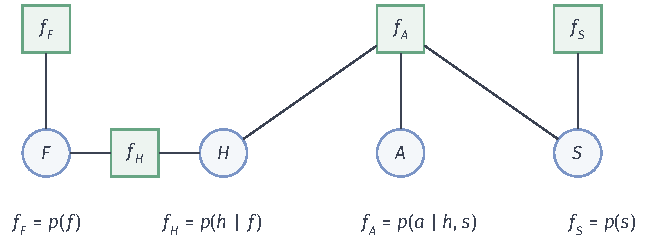
\includegraphics[width=\linewidth]{figures/03-models/03-probabilistic-graphical-models/tikz/pgm-representations-alarm-factor-graph/figure.pdf}
  \caption{报警模型的因子图。圆形是随机变量，方形是四个局部条件或先验因子。$f_H$连接$F,H$，$f_A$连接$H,A,S$；连接线表示函数输入关系，而不是有向生成边。}
  \label{fig:pgm-representations-alarm-factor-graph}
\end{figure}

对Markov网络，每个给定的势函数产生一个因子节点，连接其作用域中的变量。若输入已经细分到边势和一元势，就应保留这些小因子，而不必为每个极大团先造一张大表。反过来，把每个因子作用域中的变量两两相连，可以得到对应的无向变量图；它记录“这些变量至少共同进入一个因子”，却会忘记相互作用到底由几个因子组成。

例如，三个变量的函数$g=\psi_{\{1,2\}}\psi_{\{2,3\}}\psi_{\{1,3\}}$在无向变量图上表现为三角形，与一般的三元势$\psi_{\{1,2,3\}}$拥有相同的完整团。但前者明确承诺可分为三个二元函数，后者未必可以。无向三角形没有条件独立性可用来区分它们；因子图却能直接显示输入分解的粒度。这是计算结构提供了额外信息，而不是因子图发现了新的普通条件独立性。

\subsection{表示的非唯一性}
\label{sec:pgm-representations-nonuniqueness}

同一联合函数并不确定唯一的因子图。图~\ref{fig:pgm-representations-factor-grouping}把三个二元因子合成一个三元因子，乘积不变，因子图却从一个六边环变成星形。星形在拓扑上没有环，但中心因子的表规模已经从单个二元表的$r^2$增长到三元表的$r^3$；“图无环”不能脱离因子大小单独用作计算简单的保证。

\begin{figure}[htbp]
  \centering
  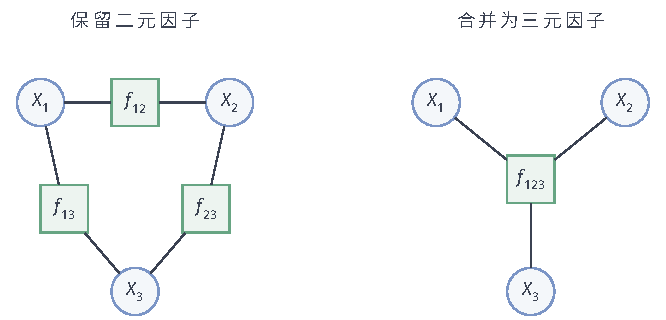
\includegraphics[width=\linewidth]{figures/03-models/03-probabilistic-graphical-models/tikz/pgm-representations-factor-grouping/figure.pdf}
  \caption{相同联合函数的两种因子图。左图保留三个二元因子，右图用$f_{123}=f_{12}f_{23}f_{13}$将其合并。两图对应的无向变量图都是三角形；因子图的环结构和因子规模却不同。}
  \label{fig:pgm-representations-factor-grouping}
\end{figure}

合并总能通过乘法进行，拆分却需要函数确实具有相应结构。对于二元变量，若$f_{12}(x_1,x_2)=u(x_1)v(x_2)$，其$2\times2$数值表的秩至多为$1$。式~\eqref{eq:pgm-representations-cycle-potentials}的表为$\left(\begin{smallmatrix}2&1\\1&2\end{smallmatrix}\right)$，行列式为$3$，所以不能拆成两个一元因子。任意三元势也不能仅因为画图方便，就声称可拆成三个二元势。

保持作用域不变，也可以通过\term{重新参数化}（reparameterization）改变局部因子，即把一部分权重从一个因子转移到另一个因子，而保持整体乘积。例如取任意严格为正的函数$h(x_2)$，令
\[
  \widetilde f_{12}=f_{12}h(x_2),\qquad
  \widetilde f_{23}=\frac{f_{23}}{h(x_2)}.
\]
两个新因子的乘积与原来完全相同。若仅把某个因子乘以正的常数，则未归一化函数$g$发生了缩放，但在同步调整$Z$后，归一化分布$p$仍相同。区分“同一联合函数”与“同一归一化分布”，有助于判断一个变换究竟保持了什么。

因子图并非完全没有独立性信息。设$A,B,S\subseteq V$两两不交，且$A,B$非空。在非负概率因子分解下，若删除一组\emph{变量节点}$S$后，$A$与$B$落在不同连通分量，则给定$\bm{X}_S=\bm{s}$后，乘积可以按这些分量分组，归一化也按组分开，从而推出$\bm{X}_A\perp\bm{X}_B\mid\bm{X}_S$。该结论只对条件分布有定义的取值$\bm{s}$使用；在有限离散情形，这要求$p(\bm{X}_S=\bm{s})>0$。但这只是充分的独立性判断，不必穷尽特定因子函数隐含的全部独立性。

报警因子图中的$H-f_A-S$一直连通，而对$a$求和有$\sum_a f_A(h,a,s)=1$，这条局部归一化约束仍能使$H$与$S$边缘独立。图拓扑自身没有记录这条等式。因此，因子图适合保存函数作用域、安排计算；要解释碰撞结构，应保留原有向图及其条件分布语义，要解释无向Markov约束，则应考察相应的无向变量图。

\subsection{因子图上的局部计算}
\label{sec:pgm-representations-local-computation}

给定证据$\bm{X}_S=\bm{s}$时，可以先把相关因子限制到该取值，再处理其余变量。设查询节点集合为$Q\subseteq V\setminus S$，其余非证据节点为$R=V\setminus(Q\cup S)$，则未归一化的边缘函数为
\begin{equation}
  \widetilde p(\bm{x}_Q,\bm{s})
  =\sum_{\bm{x}_R}
  \prod_{\alpha\in\mathcal{F}}
  f_\alpha(\bm{x}_{D_\alpha\setminus S},\bm{s}_{D_\alpha\cap S}).
  \label{eq:pgm-representations-marginal-query}
\end{equation}
在$p(\bm{s})>0$时，把$\widetilde p$除以对$\bm{x}_Q$的求和结果，即得后验边缘分布。

局部计算的依据是分配律。若因子$u$不依赖待消除变量$x_i$，则$\sum_{x_i}u\,v=u\sum_{x_i}v$，因此只需收集与$x_i$相连的因子，将它们相乘并对$x_i$求和，再把所得函数接到剩余作用域上。式~\eqref{eq:pgm-representations-cycle-message}正是这样的一次操作：两个二元因子经过消除，变为定义在$\{1,3\}$上的新因子。因子图使“收集哪些函数”“结果还依赖哪些变量”都可以由连接关系确定。

若任务是寻找全部非证据变量的最可能联合配置，则把对这些变量配置的求和改成最大化：
\[
  \max_{\bm{x}_{V\setminus S}}
  \prod_{\alpha\in\mathcal{F}}f_\alpha.
\]
这称为\term{最可能解释}（most probable explanation, MPE）。因为$Z$与待选配置无关，最大化未归一化权重即可；要恢复具体配置而不只是最大值，还必须记录局部最大化时取得最优值的变量取值，并在计算结束后回溯。若只对部分变量求最优、对其他未观测变量求和，则是边缘最大后验查询（marginal MAP），不能把所有求和都换成最大化，也不能随意交换两种消除顺序。

\term{和积}（sum-product）用乘法组合因子、用求和消除变量；\term{最大积}（max-product）保留同样的乘法组合，却用最大化消除变量。四环例子中，若在式~\eqref{eq:pgm-representations-cycle-message}里把求和改成最大值，得到的函数是：两端相同时为$4$，两端不同时为$2$，而不是原来的$5$和$4$。同一组因子服务于不同查询，区别落在消除算子上。

这两类运算可统一写成\term{半环}（semiring）上的局部计算：用$\otimes$组合局部信息，用$\oplus$汇总待消除变量的不同取值。这里使用交换半环，两个运算满足结合律与交换律，$\otimes$对$\oplus$满足分配律。再记$e_\oplus$为$\oplus$的单位元、$e_\otimes$为$\otimes$的单位元，并要求$e_\oplus$对$\otimes$具有吸收性，即$a\otimes e_\oplus=e_\oplus$。于是一个局部消除结果可写为
\begin{equation}
  \begin{aligned}
    h(\bm{x}_{D\setminus\{i\}})
    &=
    \bigoplus_{x_i}
    \ \bigotimes_{\alpha:\,i\in D_\alpha}
    f_\alpha(\bm{x}_{D_\alpha}),\\
    D&=\bigcup_{\alpha:\,i\in D_\alpha}D_\alpha.
  \end{aligned}
  \label{eq:pgm-representations-semiring-elimination}
\end{equation}
在非负实数上，$(\oplus,\otimes)=(+,\times)$给出和积，此时$(e_\oplus,e_\otimes)=(0,1)$；$(\max,\times)$给出最大积，两个单位元仍为$0$与$1$。取对数后，值域变为$\mathbb{R}\cup\{-\infty\}$，最大积可改写为$(\max,+)$形式，此时$(e_\oplus,e_\otimes)=(-\infty,0)$，零权重对应$-\infty$。把具体运算代入同一个半环表达式，便能检验分配律为何允许相同的局部消除步骤；这种统一来自代数结构，而不是图中箭头的方向\scite{pgm-overview-kschischang2001}

一次消除产生的是剩余变量上的函数，不只是一个标量。把这样概括局部子问题的函数沿图传递，就是消息传递的基本计算单位。在无环因子图上，移除一条边会把计算分成两个不重叠的部分，消息可以概括其中一侧对另一侧的作用，和积因而能精确求边缘。若在有环因子图上反复应用同样的局部消息更新，传回的信息可能已经包含当前节点先前发出的影响，不再具有这种不重叠保证；这就是后文环置信传播所面对的问题。另一条精确路线是先按消除序组合因子，再把形成的大团组织成适合消息传递的结构。第~\ref{chap:pgm-elimination}章将展开变量消除的顺序与复杂度，第~\ref{chap:pgm-junction-tree}章再说明如何组织和复用消息。

\section{本章小结}
\label{sec:pgm-representations-summary}

转换图表示时，“保留分布”“保留图独立性”和“保留计算结构”是三个不同要求。I-map只要求图声明的独立性属于分布真实独立性，即$\mathcal{I}(\mathcal{G})\subseteq\mathcal{I}(p)$；D-map的包含方向相反。针对一个查询，先取相关祖先再道德化，可以精确复现d-分离；将整个有向图一次性道德化，则通常只得到一个较弱的独立性描述。碰撞结构与无弦四环分别展示了两类图不能相互完美表达的情形，弦图和完美有向图则刻画了无向图可以无损保留图独立性的边界。

祖先道德图上的因子分组证明了d-分离的可靠性；离散条件表与线性高斯参数的非平凡多项式构造，则证明了相对于这两个模型类的完备性。完备性只保证每项未分离查询都存在一个不独立的相容分布；若要让某个固定分布中的条件独立都能反推出d-分离，还需要该分布忠实于图。

因子层面的要求较弱：有向图的条件分布可以直接作为道德图上的团因子，弦图的势函数可以沿完美消除序重组为条件分布，非弦图也能借助填充边完成精确转换。四环的数值推导说明，新图中多出的边不会自动破坏原分布已有的独立性；它只是使这些独立性不再由新图保证。把新条件表全部当成自由参数，才会扩大允许的模型族。

因子图保留的是变量与函数之间的输入关系。它既能承接有向分解，也能承接无向分解，并把求边缘与找最优配置归结为“组合局部因子，再消去变量”。同一分布可以有多种因子图，计算代价既受连接结构影响，也受因子作用域大小影响。接下来的问题因此不是寻找一种在所有方面都优于其他表示的图，而是在给定因子和查询后，选择怎样的消除顺序，才能避免生成不必要的大表。
